\section{Auswertung}
\label{sec:Auswertung}

%\begin{figure}
%  \centering
%  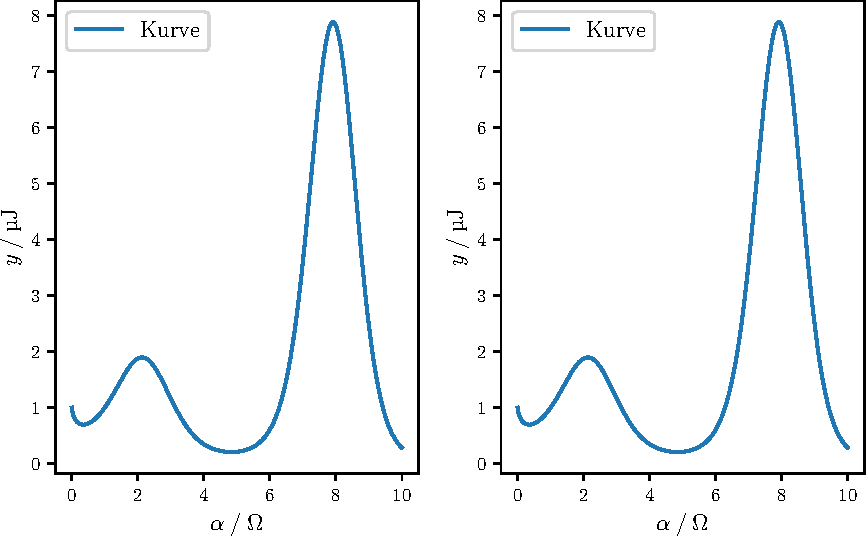
\includegraphics{plot.pdf}
%  \caption{Plot.}
%  \label{fig:plot}
%\end{figure}
%
%
%Siehe \autoref{fig:plot}!

\subsection{Bestimmung der Grenzspannung}

Um die Grenzspannung $U_G$ zu ermitteln wird die Spannung $U$ gegen die Quadratwurzel des Photostroms $I$ aufgetragen. 
Durch die linearen Abschnitte wird eine Ausgleichsgerade gezogen.
Der Schnittpunkt der Geraden mit der x-Achse entspricht der Grenzspannung $U_G$.
Mit der Ausgleichsgerade $I = a \cdot U + b$, lässt sich die Grenzspannung berechnen mit
\begin{equation*}
  U_G = - \frac{b}{a}.
\end{equation*}
\\
\\
\begin{table}[H]
  \centering
  \caption{Brems- und Beschleunigungsspannung $U$ und Photostrom $I$ bei violettem Licht.}
  \begin{tabular}{|c|c|}
    \toprule
    $U \,/\, [\si{\volt}]$ & $I \,/\, [\si{\nano\ampere}]$\\
    \midrule
    -1.99 & 0\\
    -1.90 & 0\\
    -1.70 & 0\\
    -1.50 & 0\\
    -1.30 & 0\\
    -1.10 & 0\\
    -1.05 & 0\\
    -1.00 & 0.009\\
    -0.95 & 0.026\\
    -0.90 & 0.046\\
    -0.85 & 0.070\\
    -0.80 & 0.098\\
    -0.75 & 0.130\\
    -0.70 & 0.160\\
    -0.65 & 0.210\\
    -0.60 & 0.250\\
    -0.55 & 0.320\\
    -0.50 & 0.370\\
    -0.45 & 0.420\\
    -0.40 & 0.480\\
    -0.35 & 0.540\\
    -0.30 & 0.580\\
    \bottomrule
  \end{tabular}
  \begin{tabular}{|c|c|}
    \toprule
    $U \,/\, [\si{\volt}]$ & $I \,/\, [\si{\nano\ampere}]$\\
    \midrule
    -0.25 & 0.620\\
    -0.20 & 0.670\\
    -0.15 & 0.720\\
    -0.10 & 0.760\\
    -0.05 & 0.810\\
    -0.01 & 0.860\\
    0.05 & 0.900\\
    0.10 & 0.940\\
    0.15 & 0.980\\
    0.20 & 1.000\\
    0.25 & 1.000\\
    0.30 & 1.100\\
    0.40 & 1.200\\
    0.50 & 1.200\\
    0.70 & 1.400\\
    0.90 & 1.500\\
    1.10 & 1.600\\
    1.30 & 1.800\\
    1.50 & 1.900\\
    1.70 & 2.100\\
    1.90 & 2.300\\
    1.99 & 2.400\\
    \bottomrule
  \end{tabular}
  \label{tab:lila}
\end{table}

\begin{table}
  \centering
  \caption{Brems- und Beschleunigungsspannung $U$ und Photostrom $I$ bei grünem Licht.}
  \begin{tabular}{|c|c|}
    \toprule
    $U \,/\, [\si{\volt}]$ & $I \,/\, [\si{\nano\ampere}]$\\
    \midrule
    -1.99 & 0\\
    -1.90 & 0\\
    -1.80 & 0\\
    -1.70 & 0\\
    -1.60 & 0\\
    -1.50 & 0\\
    -1.20 & 0\\
    -1.00 & 0\\
    -0.80 & 0\\
    -0.60 & 0\\
    -0.55 & 0.010\\
    -0.50 & 0.028\\
    -0.45 & 0.055\\
    -0.40 & 0.094\\
    -0.35 & 0.140\\
    -0.30 & 0.200\\
    -0.25 & 0.260\\
    -0.20 & 0.300\\
    -0.15 & 0.350\\
    \bottomrule
  \end{tabular}
  \begin{tabular}{|c|c|}
    \toprule
    $U \,/\, [\si{\volt}]$ & $I \,/\, [\si{\nano\ampere}]$\\
    \midrule
    -0.10 & 0.400\\
    -0.05 & 0.440\\
    -0.01 & 0.470\\
    0.05 & 0.520\\
    0.10 & 0.540\\
    0.15 & 0.580\\
    0.20 & 0.600\\
    0.30 & 0.680\\
    0.40 & 0.740\\
    0.50 & 0.790\\
    0.60 & 0.840\\
    0.70 & 0.900\\
    0.80 & 0.960\\
    0.90 & 1.000\\
    1.20 & 1.150\\
    1.40 & 1.200\\
    1.60 & 1.200\\
    1.80 & 1.400\\
    1.99 & 1.600\\
    \bottomrule
  \end{tabular}
  \label{tab:gruen}
\end{table}

\begin{table}
  \centering
  \caption{Brems- und Beschleunigungsspannung $U$ und Photostrom $I$ bei gelbem Licht.}
  \begin{tabular}{|c|c|}
    \toprule
    $U \,/\, [\si{\volt}]$ & $I \,/\, [\si{\nano\ampere}]$\\
    \midrule
    -19.00 & 0\\
    -5.00 & 0\\
    -1.00 & 0\\
    -0.50 & 0\\
    -0.01 & 0\\
    0.01 & 0.22\\
    0.50 & 0.40\\
    1.00 & 0.55\\
    1.50 & 0.68\\
    2.00 & 0.82\\
    2.50 & 0.97\\
    3.00 & 1.00\\
    3.50 & 1.20\\
    4.00 & 1.20\\
    5.00 & 1.40\\
    \bottomrule
  \end{tabular}
  \begin{tabular}{|c|c|}
    \toprule
    $U \,/\, [\si{\volt}]$ & $I \,/\, [\si{\nano\ampere}]$\\
    \midrule
    6.00 & 1.40\\
    7.00 & 1.55\\
    8.00 & 1.60\\
    9.00 & 1.70\\
    10.0 & 1.80\\
    11.0 & 1.80\\
    12.00 & 1.85\\
    13.00 & 1.95\\
    14.00 & 2.00\\
    15.00 & 2.00\\
    16.00 & 2.00\\
    17.00 & 2.10\\
    18.00 & 2.20\\
    19.00 & 2.20\\
    \text{---} & \text{---}\\
    \bottomrule 
  \end{tabular}
  \label{tab:gelb}
\end{table}

\begin{table}
  \centering
  \caption{Brems- und Beschleunigungsspannung $U$ und Photostrom $I$ bei rotem Licht.}
  \begin{tabular}{|c|c|}
    \toprule
    $U \,/\, [\si{\volt}]$ & $I \,/\, [\si{\nano\ampere}]$\\
    \midrule
    -1.99 & 0\\
    -1.00 & 0\\
    -0.70 & 0\\
    -0.65 & 0\\
    -0.60 & 0\\
    -0.55 & 0.001\\
    -0.50 & 0.002\\
    -0.45 & 0.002\\
    -0.40 & 0.003\\
    -0.35 & 0.004\\
    -0.30 & 0.004\\
    -0.25 & 0.006\\
    -0.20 & 0.008\\
    -0.10 & 0.011\\
    -0.01 & 0.014\\
    \bottomrule
  \end{tabular}
  \begin{tabular}{|c|c|}
    \toprule
    $U \,/\, [\si{\volt}]$ & $I \,/\, [\si{\nano\ampere}]$\\
    \midrule
    0.10 & 0.018\\
    0.20 & 0.022\\
    0.30 & 0.026\\
    0.40 & 0.029\\
    0.50 & 0.032\\
    0.60 & 0.035\\
    0.70 & 0.038\\
    0.80 & 0.042\\
    1.00 & 0.048\\
    1.20 & 0.052\\
    1.40 & 0.057\\
    1.60 & 0.062\\
    1.80 & 0.066\\
    1.99 & 0.072\\
    \text{---} & \text{---}\\
    \bottomrule
  \end{tabular}
  \label{tab:rot}
\end{table}